\documentclass[12pt,a4paper]{article}

% Packages
\usepackage{amsmath, amssymb}
\usepackage{graphicx}
\usepackage{siunitx} 
\usepackage{caption}
\usepackage{geometry}
\usepackage{hyperref}
\usepackage{url}
\usepackage{cite}
\usepackage{listings}
\usepackage{listings-rust}
\usepackage{xurl}
\usepackage{siunitx}
\usepackage{tikz}

\lstset{language=Rust, style=boxed}
\geometry{margin=1in}
\graphicspath{{/images}}

\title{Sensors and Actuators for Robotics and
Automation\\Term Project Progress Report III}
\author{Kanisorn Sangchai (ID: 6538020621)}
\date{October 20, 2025}

\begin{document}

\maketitle

\section{Introduction}
This report documents the implementation of Analog-to-Digital Conversion, software configuration, and sensor value read for a thermistor-based temperature sensor system. The STM32H743VIT6 core board by WeAct Studio is used to perform the analog to digital conversion and transmit the measured sensor values via UART communication. The source code for this project can be found in this GitHub repository: \url{https://github.com/Kanisorn-S/sara-project}. The source code for Milestone 2 can be found in the \texttt{Milestone-3} branch: \url{https://github.com/Kanisorn-S/sara-project/tree/Milestone-3}.

\begin{figure}[h]
    \centering
    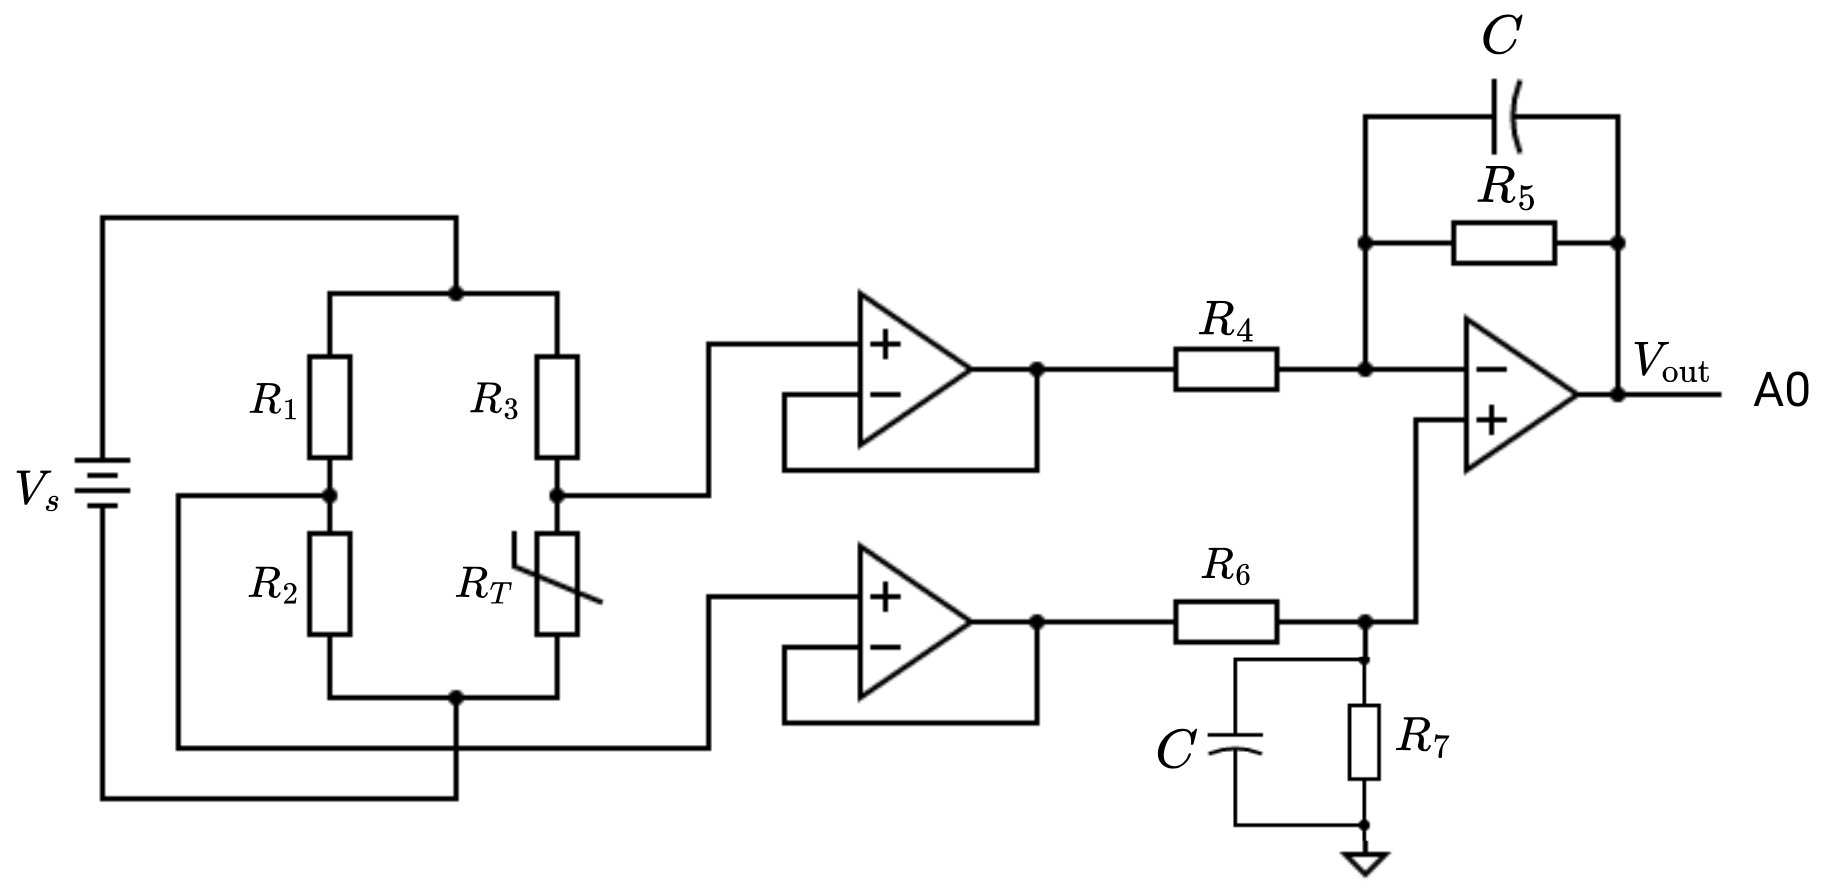
\includegraphics[width=0.9\textwidth]{images/circuit_diagram.png}
    \caption{Original circuit diagram with an adjustable voltage divider added to control the temperature}
    \label{fig:circuit}
\end{figure}

\begin{figure}[h]
  \centering
  \begin{tikzpicture}
    \node[anchor=south west, inner sep=0] (img) {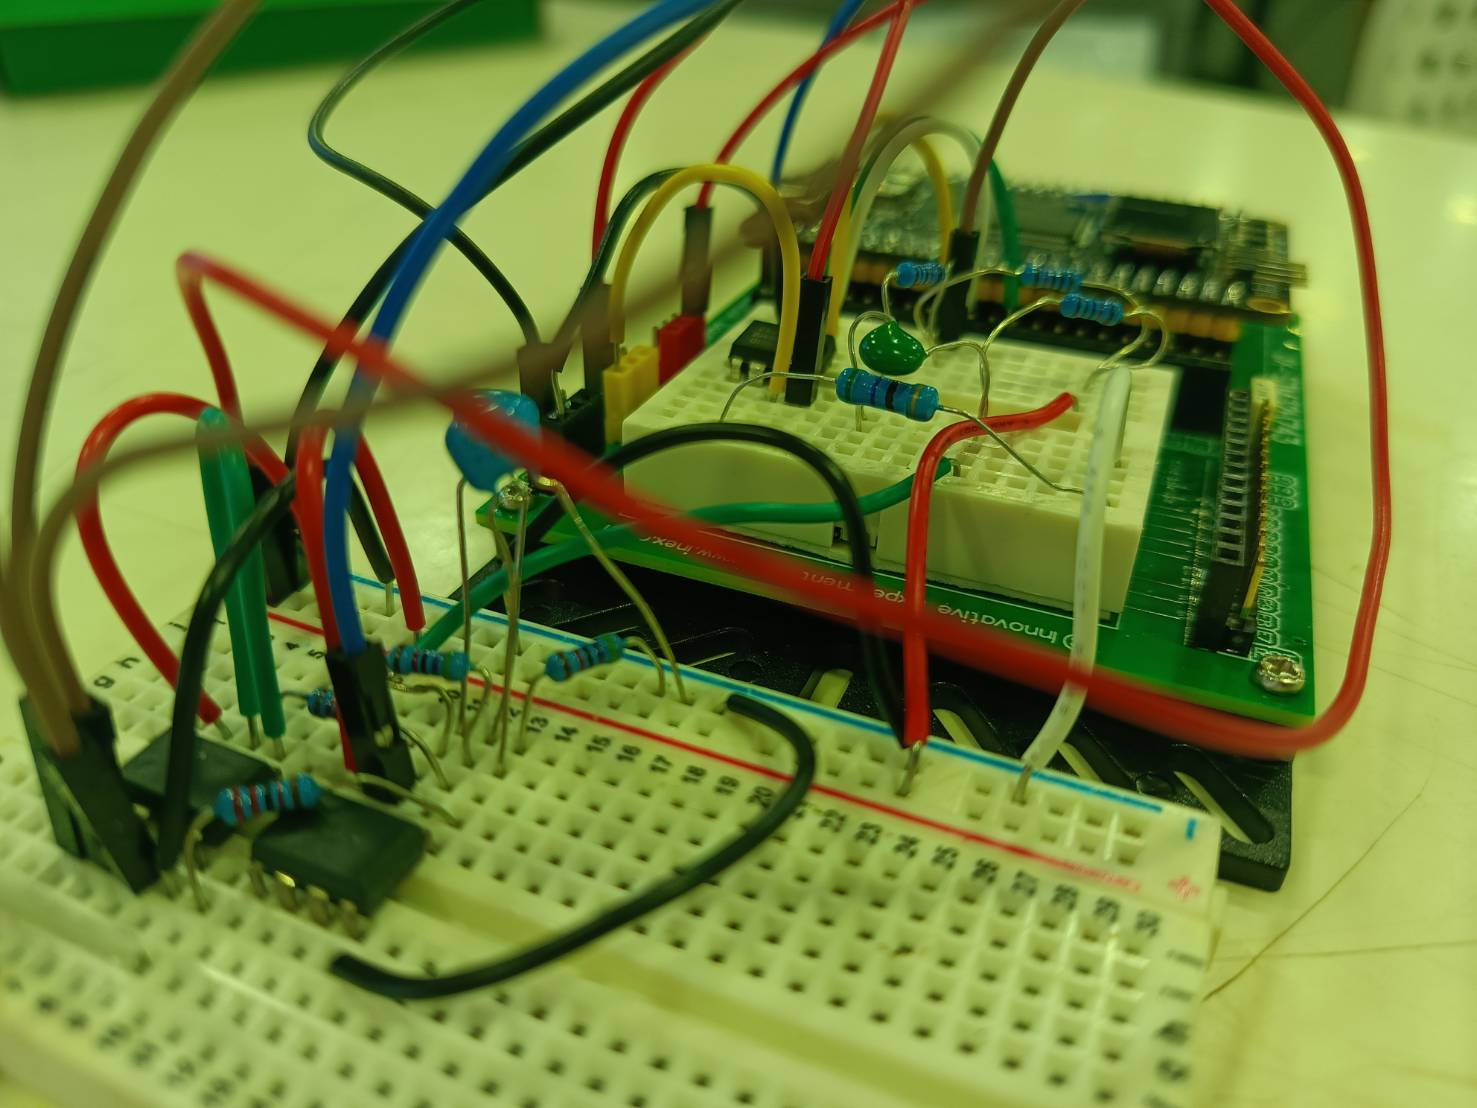
\includegraphics[width=0.9\linewidth]{images/actual_circuit.jpg}};
    \begin{scope}[x={(img.south east)}, y={(img.north west)}]
      % Example markers (adjust coordinates)
      \draw[red, line width=5pt, rounded corners] (0.65,0.6) rectangle (0.55,0.74);
      \node[red, fill=white, font=\small, align=center] at (0.75,0.90) {Thermistor and adjacent fixed resistor};

      % Optional arrows
      \draw[->, line width=2pt, red] (0.75,0.87) -- (0.65,0.74);
    \end{scope}
  \end{tikzpicture}
  \caption{Physical implementation of the circuit showing the thermistor and the adjacent fixed resistor (highlighted) used in the adjustable voltage divider for temperature control.}
  \label{fig:actual-circuit}
\end{figure}


\section{Circuit Design}
An adjustable voltage divider was added to the original circuit design, as shown in Figure~\ref{fig:circuit}, to manipulate the temperature of the thermistor. In the physical implementation shown in Figure~\ref{fig:actual-circuit}, the fixed resistor of the voltage divider is positioned adjacent to the thermistor so that changes in the resistor’s temperature directly influence the thermistor’s resistance.

The voltage divider consists of 
\begin{itemize}
    \item Potentiometer
    \item Fixed Resistor
\end{itemize} 
By adjusting the potentiometer, the voltage across the fixed resistor can be changed, which in turn changes its temperature.

\subsection{Components}
\subsubsection{Potentiometer}
For this project, a digital potentiometer is used to adjust the voltage divider ratio, thus adjusting the voltage across the fixed resistor. The voltage across the fixed resistor $V_{\text{Heat}}$ can be calculated using the formula:

\begin{equation*}
    V_{\text{Heat}} = V_s \cdot \frac{R_{\text{Fixed}}}{R_{\text{Fixed}} + R_{\text{Pot}}}
\end{equation*}

Where:

\begin{equation*}
    R_{\text{Pot}} = R_{\text{Pot, Max}} \cdot \frac{\text{pot\_value}}{\text{pot\_value}_{\text{Max}}}
\end{equation*}

Giving us:

\begin{equation}
    \label{eq:v-heat-theta}
    V_{\text{Heat}} = V_s \cdot \frac{R_{\text{Fixed}}}{R_{\text{Fixed}} + R_{\text{Pot, Max}} \cdot \frac{\text{pot\_value}}{\text{pot\_value}_{\text{Max}}}}
\end{equation}

The selected potentiometer is the MCP41010 Single Digital Potentiometer with 256 taps and a maximum resistance of $\SI{10}{k\ohm}\pm 20\%$~\cite{potentiometer},\cite{pot-tolerance}.

\subsubsection{Fixed Resistor}
For this project, a fixed resistor is used in conjunction with the potentiometer to form the voltage divider. The value of the fixed resistor $R_{\text{Heat}}$ is chosen to be $\SI{560}{\ohm}\pm 1\%$. This value is selected to ensure that the voltage across the fixed resistor can be adjusted within a suitable range for heating purposes.

\section{Mathematical Model}

\subsection{Temperature Manipulation}
We use our STM32H743VIT6 Core Board's \SI{3.3}{\volt} to power the adjustable voltage divider, giving us $V_s=\SI{3.3}{\volt}$. To manipulate the temperature of the thermistor, we can set the value $\text{pot\_value}$ of the potentiometer. From Equation~\eqref{eq:v-heat-theta}, we can see that the maximum voltage across the fixed resistor occurs when $\text{pot\_value} = 0$, which gives us:
\begin{equation*}
    V_{\text{Heat, Min}} = V_s \cdot \frac{R_{\text{Fixed}}}{R_{\text{Fixed}} + 0} = V_s = \SI{3.3}{\volt}
\end{equation*}
While the minimum voltage occurs when $\text{pot\_value} = \text{pot\_value}_{\text{Max}}$, which gives us:
\begin{equation*}
    V_{\text{Heat, Max}} = V_s \cdot \frac{R_{\text{Fixed}}}{R_{\text{Fixed}} + R_{\text{Pot, Max}}} = \SI{3.3}{\volt} \cdot \frac{\SI{560}{\ohm}}{\SI{560}{\ohm} + \SI{10}{k\ohm}} = \SI{0.175}{\volt}
\end{equation*}
Calculating for the error,
\begin{align*}
    \frac{\delta V_{\text{Heat}}}{V_{\text{Heat}}} &=  \frac{\delta R_\text{fixed}}{R_\text{fixed}} + \frac{\delta (R_\text{fixed} + R_\text{pot})}{R_\text{fixed} + R_\text{pot}} \\
    &= 0.01 + \frac{0.01 \cdot R_\text{fixed} + 0.2 \cdot R_\text{pot}}{R_\text{fixed} + R_\text{pot}} \\
    &= 0.01 + \frac{0.01 \cdot 560 + 0.2 \cdot 10000}{560 + 10000} \\
    &\approx 0.01 + 0.19 \\
    &\approx 0.2
\end{align*}

\begin{table}[h!]
\centering
\begin{tabular}{lccc}
\hline
\textbf{DIN size} & \textbf{0204} & \textbf{0207} & \textbf{0414} \\
\hline
Thermal time constant, $\tau_w$ (s) & 2 & 5 & 20 \\
Thermal resistance, $R_{th}$ (K/W)  & 400 & 250 & 170 \\
\hline
\end{tabular}
\caption{Examples of resistor thermal time constant and thermal resistance on leaded cylindrical components. (from~\cite{thermal-resistance})}
\label{tab:thermal-resistance}
\end{table}

To find the change in temperature of the fixed resistor based on the voltage across it, we first need to find the resistor's thermal resistance $R_{\text{th}}$. Our resistor's body length is $\SI{10}{mm}$, the closest DIN standard size to our resistor's body length is 0414~\cite[pp.~13]{din}. From Table~\ref{tab:thermal-resistance}, we can find that the thermal resistance for a 0414 resistor is $R_{\text{th}} = \SI{170}{K/W}$. The temperature change $\Delta T$ of the fixed resistor can be calculated using the formula:
\begin{equation*}
    \Delta T = R_{\text{th}} \cdot P
\end{equation*}
Where $P$ is the power dissipated by the resistor, which can be calculated using the formula:
\begin{equation*}
    P = \frac{V_{\text{Heat}}^2}{R_{\text{Heat}}}
\end{equation*}
Combining the two equations, we get:
\begin{equation}
    \Delta T = R_{\text{th}} \cdot \frac{V_{\text{Heat}}^2}{R_{\text{Heat}}}
    \label{eq:delta-t}
\end{equation}
To get the full equation, we combine Equation~\ref{eq:v-heat-theta} and Equation~\ref{eq:delta-t} to get:
\begin{equation}
    \Delta T = R_{\text{th}} \cdot \frac{\left(V_s \cdot \frac{R_{\text{Fixed}}}{R_{\text{Fixed}} + R_{\text{Pot, Max}} \cdot \frac{\text{pot\_value}}{\text{pot\_value}_{\text{Max}}}}\right)^2}{R_{\text{Heat}}}
    \label{eq:full-delta-t}
\end{equation}

Finally, the temperature that our sensor will be measuring is given by
\begin{align}
    T &= T_{\text{ambient}} + \Delta T \nonumber \\
      &= T_{\text{ambient}} + R_{\text{th}} \cdot \frac{\left(V_s \cdot \frac{R_{\text{Fixed}}}{R_{\text{Fixed}} + R_{\text{Pot, Max}} \cdot \frac{\text{pot\_value}}{\text{pot\_value}_{\text{Max}}}}\right)^2}{R_{\text{Heat}}} \label{eq:final-temp}
\end{align}
Where $T_{\text{ambient}}$ is a parameter of our system and must be determined before using the sensor.


\label{sec:math-model}

\subsection{Kalman Filter}
We first design the mathematical formalism of the Kalman Filter for our system. The equation for our system is

\begin{align}
    &x_k = A x_{k-1} + C + w_{k-1} \\
    &w_k \sim \mathcal{N}(0,\mathbf{Q}) \label{eq:q}
\end{align}
Where $x_k$ is the state variable at time $k$, $A$ is the state transition coefficient, $C$ is the additive component, and $w_k$ is the system process noise at time $k$.

The equation for our sensor measurement is

\begin{align}
    &z_k = H x_k + v_k \\
    &v_k \sim \mathcal{N}(0, \mathbf{R}) \label{eq:r}
\end{align}
Where $z_k$ is the sensor output at time $k$, $H$ is the sensing coefficient, and $v_k$ is the sensing noise.

Because our system is concerned only with temperature measurement, the corresponding coefficients are represented as scalars rather than matrices.

\subsubsection{State Variable $x_k$}
Because our system is concerned only with temperature measurement, the state variable $x_k$ is a single scalar value 

\begin{equation*}
    x_k = T_k
\end{equation*}

which represents the temperature of the system at time $k$.

\subsubsection{State Transition Coefficient $A$}
From Equation~\eqref{eq:final-temp}, we can control the temperature of the system $T$ by programatically adjusting the value of the digital potentiometer $\text{pot\_value}$. Since the temperature of the system at any given time is only dependent on the current setting of the potentiometer and not on the previous temperature, the state transition coefficient $A$ is

\begin{equation*}
    A = 0
\end{equation*}

\subsubsection{Additive Component $C$}
From Equation~\eqref{eq:final-temp}, we can control the temperature of the system $T$ by programatically adjusting the value of the digital potentiometer $\text{pot\_value}$; therefore, the additive component $C$ is given by

\begin{equation*}
    C = T_{\text{ambient}} + R_{\text{th}} \cdot \frac{\left(V_s \cdot \frac{R_{\text{Fixed}}}{R_{\text{Fixed}} + R_{\text{Pot, Max}} \cdot \frac{\text{pot\_value}}{\text{pot\_value}_{\text{Max}}}}\right)^2}{R_{\text{Heat}}}
\end{equation*}

\subsubsection{Sensing Coefficient $H$}
Since our sensor is measuring the temperature, which is the value we want to know, the sensing coefficient $H$ is simply

\begin{equation*}
    H = 1
\end{equation*}

\subsubsection{Process Covariance $Q$}
From Equation~\eqref{eq:q}, $Q$ is the covariance of our system process noise $w_k$. We can calculate this by taking multiple temperature measurements for multiple states of our system (multiple different $\text{pot\_value}$) using a trustworthy digital thermometer then finding the covariance using


\begin{equation}
    \label{eq:cov}
    \mathrm{Cov}(X) = \frac{1}{N} \sum_{i=1}^{N} (X_i - \mu_X)^2
\end{equation}

Twenty temperature measurements were recorded using a reliable digital thermometer positioned near the thermistor, as shown in Figure~\ref{fig:measure-temp}, for each of the following 15 $\text{pot\_value}$

\begin{equation}
    \label{eq:pot-value}
    \text{pot\_value} = 0, 17, 34, 51, 68, 85, 102, 119, 136, 153, 170, 187, 204, 221, 238, 255
\end{equation}

From the result recorded in our \href{https://docs.google.com/spreadsheets/d/1mIqAQL7zom7rqrgY63SVOOFBYus10Tk0CKpmR08Oij0/edit?gid=0#gid=0}{\textbf{\underline{Google Sheet}}}
, we can find $Q$ by using Equation~\eqref{eq:cov} for each $\text{pot\_value}$ setting, where 

\begin{itemize}
    \item $N=20$ for the 20 readings we took for each $\text{pot\_value}$
    \item $X_i$ is each of the temperature reading from the \textbf{digital thermometer}
    \item $\mu_X$ is the mean of the temperature readings from the \textbf{digital thermometer}
\end{itemize}
then finding the geometric average over all the $\text{pot\_value}$ using
\begin{equation}
    \label{eq:geo-avg}
    \bar{x}_{\mathrm{geo}} = \left( \prod_{i=1}^{N} x_i \right)^{\tfrac{1}{N}}
\end{equation}
where
\begin{itemize}
    \item $N=16$ for the 16 different $\text{pot\_value}$ settings
    \item $x_i$ is the covariance calculated using Equation~\eqref{eq:cov} for each $\text{pot\_value}$
    \item $\bar{x}_{\mathrm{geo}}=Q$
\end{itemize}
This gives us
\begin{align*}
    Q = \SI{0.0028}{\degreeCelsius^2}
\end{align*}

\subsubsection{Sensor Noise Covariance $R$}
From Equation~\eqref{eq:r}, $R$ is the covariance of our sensor noise $v_k$. We can calculate this by taking multiple temperature measurements for multiple states of our system (multiple different $\text{pot\_value}$) using both a trustworthy digital thermometer and our temperature sensor then finding the covariance using Equation~\eqref{eq:cov}.

Twenty temperature measurements were recorded for each of the $\text{pot\_value}$ in~\eqref{eq:pot-value}
From the result recorded in our \href{https://docs.google.com/spreadsheets/d/1mIqAQL7zom7rqrgY63SVOOFBYus10Tk0CKpmR08Oij0/edit?gid=501799072#gid=501799072}{\textbf{\underline{Google Sheet}}}, we can find $R$ by using Equation~\eqref{eq:cov} for each $\text{pot\_value}$ setting, where

\begin{itemize}
    \item $N=20$ for the 20 readings we took for each $\text{pot\_value}$
    \item $X_i$ is each of the temperature reading from \textbf{our temperature sensor}
    \item $\mu_X$ is the ground truth temperature reading from the \textbf{digital thermometer}
\end{itemize}
then finding the geometric average over all the $\text{pot\_value}$ using Equation~\eqref{eq:geo-avg}, where
\begin{itemize}
    \item $N=16$ for the 16 different $\text{pot\_value}$ settings
    \item $x_i$ is the covariance calculated using Equation~\eqref{eq:cov} for each $\text{pot\_value}$
    \item $\bar{x}_{\mathrm{geo}}=R$
\end{itemize}
This gives us
\begin{align*}
    R = \SI{0.395}{\degreeCelsius^2}
\end{align*}

\section{Demonstration and Verification}

\section{Conclusion}


\newpage
\bibliographystyle{IEEEtran}
\bibliography{ref}

\end{document}
